% Intrinsic growth rate r and mean generation interval T_g of Marburg
% outbreaks over time (data: outbreak_r_tg_timeline.csv).
% Top panel: r (day^-1) with 95% CI, for outbreaks with an estimable growth
% phase. Bottom panel: mean serial interval T_g from reconstructed transmission
% pairs (error bar = pair SD where n>1), against the pooled Marburg estimate
% (Qian et al. 2023, 9.2 +/- 4.4 d). Okabe-Ito colorblind-safe palette.
% Compile with pdflatex/lualatex + pgfplots (>= 1.16).
\documentclass[border=3pt]{standalone}
\usepackage{pgfplots}
\usepackage{pgfplotstable}
\usepgfplotslibrary{groupplots}
\pgfplotsset{compat=1.16}

\definecolor{oiOrange}{RGB}{230,159,0}
\definecolor{oiGreen}{RGB}{0,158,115}
\definecolor{oiBlue}{RGB}{0,114,178}
\definecolor{oiVermil}{RGB}{213,94,0}
\definecolor{oiBlack}{RGB}{0,0,0}
\definecolor{oiSky}{RGB}{86,180,233}
\definecolor{oiPurple}{RGB}{204,121,167}

% \rpt{year}{r}{lo}{hi}{color}{label}{labeldx}
\newcommand{\rpt}[7]{%
  \draw[#5,line width=1.3pt] (axis cs:#1,#3) -- (axis cs:#1,#4);%
  \fill[#5] (axis cs:#1,#2) circle (2.6pt);%
  \node[#5,font=\scriptsize,anchor=west] at (axis cs:{#1+#7},#2) {#6};}
% \tpt{year}{tg}{sd}{color}{label}  (sd=0 -> no bar)
\newcommand{\tpt}[5]{%
  \draw[#4,line width=1.3pt] (axis cs:#1,{#2-#3}) -- (axis cs:#1,{#2+#3});%
  \fill[#4] (axis cs:#1,#2) circle (2.6pt);%
  \node[#4,font=\scriptsize,anchor=west] at (axis cs:{#1+0.6},#2) {#5};}

\begin{document}
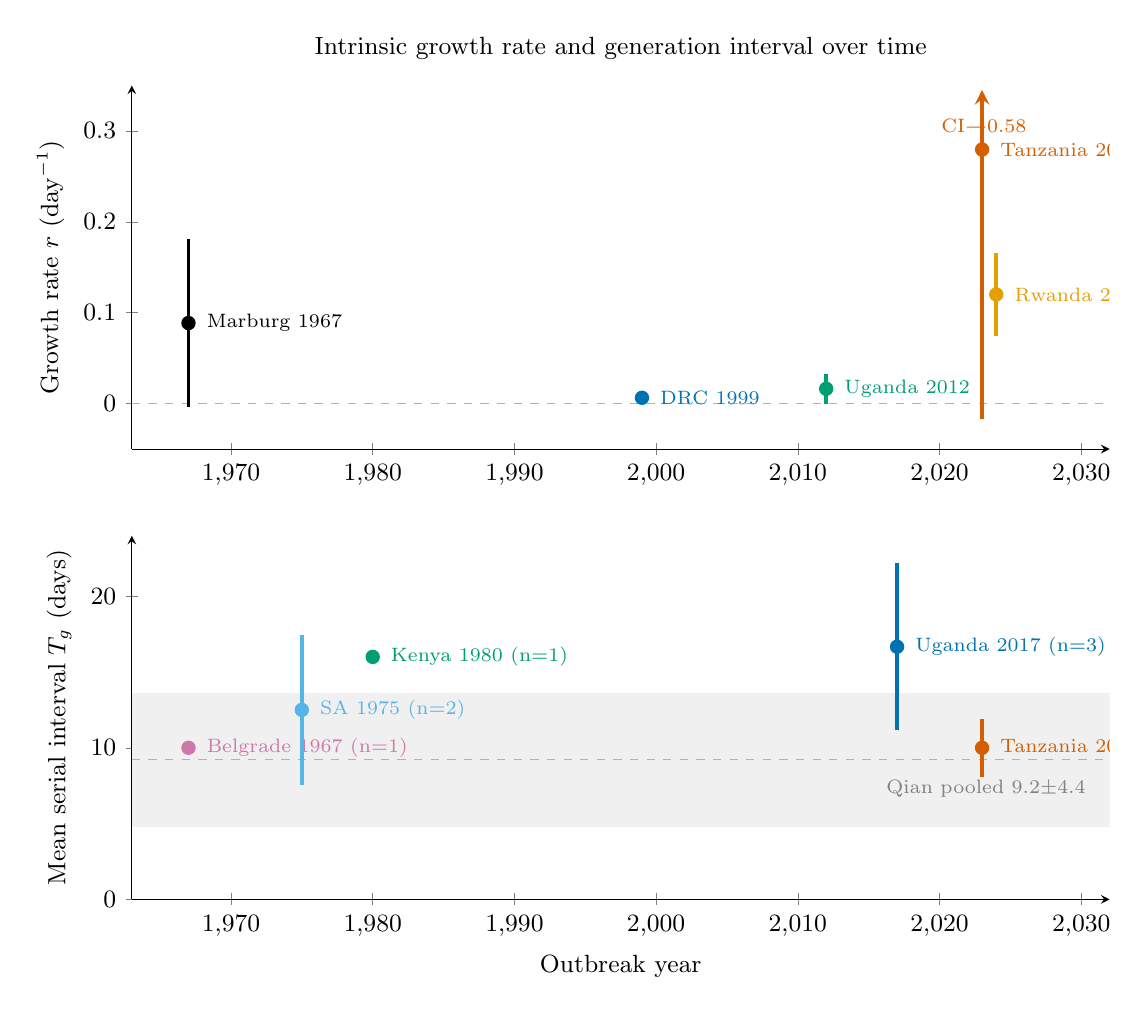
\begin{tikzpicture}
\begin{groupplot}[group style={group size=1 by 2, vertical sep=1.1cm},
    width=14cm, height=6.2cm, xmin=1963, xmax=2032,
    xtick={1970,1980,1990,2000,2010,2020,2030},
    tick label style={font=\small}, label style={font=\small}, axis lines=left]

% ---------- top: growth rate ----------
\nextgroupplot[ymin=-0.05, ymax=0.35, ylabel={Growth rate $r$ (day$^{-1}$)},
    title={\small Intrinsic growth rate and generation interval over time}]
\draw[gray!60,dashed] (axis cs:1963,0) -- (axis cs:2032,0);
\rpt{1967}{0.0886}{-0.0036}{0.1808}{oiBlack}{Marburg 1967}{0.6}
\rpt{1999}{0.0064}{0.0015}{0.0113}{oiBlue}{DRC 1999}{0.6}
\rpt{2012}{0.0163}{-0.0003}{0.0329}{oiGreen}{Uganda 2012}{0.6}
% Tanzania 2023: upper CI 0.575 off-panel (arrow)
\draw[oiVermil,line width=1.3pt] (axis cs:2023,-0.0164) -- (axis cs:2023,0.32);
\draw[oiVermil,-stealth,line width=1.3pt] (axis cs:2023,0.32) -- (axis cs:2023,0.345);
\fill[oiVermil] (axis cs:2023,0.2795) circle (2.6pt);
\node[oiVermil,font=\scriptsize,anchor=west] at (axis cs:2023.6,0.2795){Tanzania 2023};
\node[oiVermil,font=\scriptsize] at (axis cs:2023,0.305){\,CI$\to$0.58};
\rpt{2024}{0.1201}{0.0743}{0.1658}{oiOrange}{Rwanda 2024}{0.6}

% ---------- bottom: generation interval ----------
\nextgroupplot[ymin=0, ymax=24, ylabel={Mean serial interval $T_g$ (days)},
    xlabel={Outbreak year}]
\fill[gray!12] (axis cs:1963,4.8) rectangle (axis cs:2032,13.6);
\draw[gray!60,dashed] (axis cs:1963,9.2) -- (axis cs:2032,9.2);
\node[gray,font=\scriptsize,anchor=east] at (axis cs:2031,7.3){Qian pooled 9.2$\pm$4.4};
\tpt{1967}{10.0}{0}{oiPurple}{Belgrade 1967 (n=1)}
\tpt{1975}{12.5}{4.95}{oiSky}{SA 1975 (n=2)}
\tpt{1980}{16.0}{0}{oiGreen}{Kenya 1980 (n=1)}
\tpt{2017}{16.67}{5.51}{oiBlue}{Uganda 2017 (n=3)}
\tpt{2023}{10.0}{1.91}{oiVermil}{Tanzania 2023 (n=7)}
\end{groupplot}
\end{tikzpicture}
\end{document}
